%\documentclass[journal]{IEEEtran}
\documentclass[conference]{IEEEtran}
%\documentclass[twocolumn]{article}

% Begin IEEE recommended very useful LaTeX packages:
\usepackage{cite}
\usepackage{graphicx}
\usepackage{epsfig}
\usepackage{psfrag}
\usepackage{subfigure}
\usepackage{url}  
\usepackage{array}
\usepackage{amsmath}
\interdisplaylinepenalty=2500
% End IEEE recommended very useful LaTeX packages:

\usepackage{verbatim}

\newcommand{\var}[1]{{\footnotesize #1}}

% correct bad hyphenation here
\hyphenation{op-tical net-works semi-conduc-tor IEEEtran}

\newcommand{\email}[1]{\textless #1\textgreater}
\newcommand{\img}[4][width=\linewidth]
{
\begin{figure}[ht]
\centering
\includegraphics[#1]{#2}
\caption{#3}
\label{#4}
\end{figure}
}

\newcommand{\pmv}{pMarineViewer}
%\newcommand{\bhvsg}{bhv\_SearchGrid}
%\newcommand{\helm}{IvP Helm}
%\newcommand{\phelm}{pHelmIvP}
%\newcommand{\ibuff}{info\_buffer}
%\newcounter{listing}
%\newcounter{alisting}

\newlength{\pin}
\setlength{\pin}{0.2in}
\newenvironment{hangpar}[1]{\list{}{
    \setlength{\listparindent}{1.5em}       \setlength{\itemindent}{0pt}
    \setlength{\itemsep}{0pt}               \setlength{\parindent}{0pt}
    \setlength{\rightmargin}{0pt}           \setlength{\leftmargin}{#1}
               \parsep                                 \medskipamount}%
    \item\hspace{-\leftmargin}\noindent\ignorespaces}
    {\endlist}


\begin{document}
\title{A Guide to MOOSIvP Graphical Tools}
\author{Andrew Shafer, Michael Benjamin \\
Dept of Electrical Engineering/Computer Science, MIT \\
Cambridge MA 02139 \\
\email{ajshafer@mit.edu}, \email{mikerb@mit.edu} \\ \\
{\Large{\today}}}
\maketitle


\begin{abstract}
Documentation for some of the MOOS/IvP graphical tools, including pMarineViewer and polyview.  Includes instructions for clients using the tools and for programmers who want to use more advanced features.
\end{abstract}

\section{Introduction}
\label{intro}

This document describes the use and development of the artifact search system developed as a Master's of Engineering thesis by Andrew Shafer at MIT.  This document assumes that the reader has a familiarity with MOOS and IvP and understands how to use those tools (see \cite{new03}, \cite{ben02a}, \cite{ben03}, and \cite{ben04b}).

First, a bit of terminology.  In this document, an "artifact" is an object of interest.  An artifact can be any detectable, identifiable object.  In a naval application this would commonly be some type of mine.  In naval terminology, "mine-hunting" (or mine-sweeping) usually refers to the process of detecting mines and deactivating or destroying them.  "Mine-searching," on the other hand, refers to simply mapping out the locations of detected mines for later deactivation/destruction.  Therefore, this project is more properly an artifact searching system, rather than a mine-hunting system.

A "search area" is the geographic region that the user desires to search (see Figure~\ref{searcharea}).  This area is broken up into uniform, discrete cells that together constitute the "search grid" (see Figure~\ref{searchgrid}).

\begin{figure}[ht]
\label{searcharea}
\begin{minipage}[c]{0.5\textwidth}
  \centering 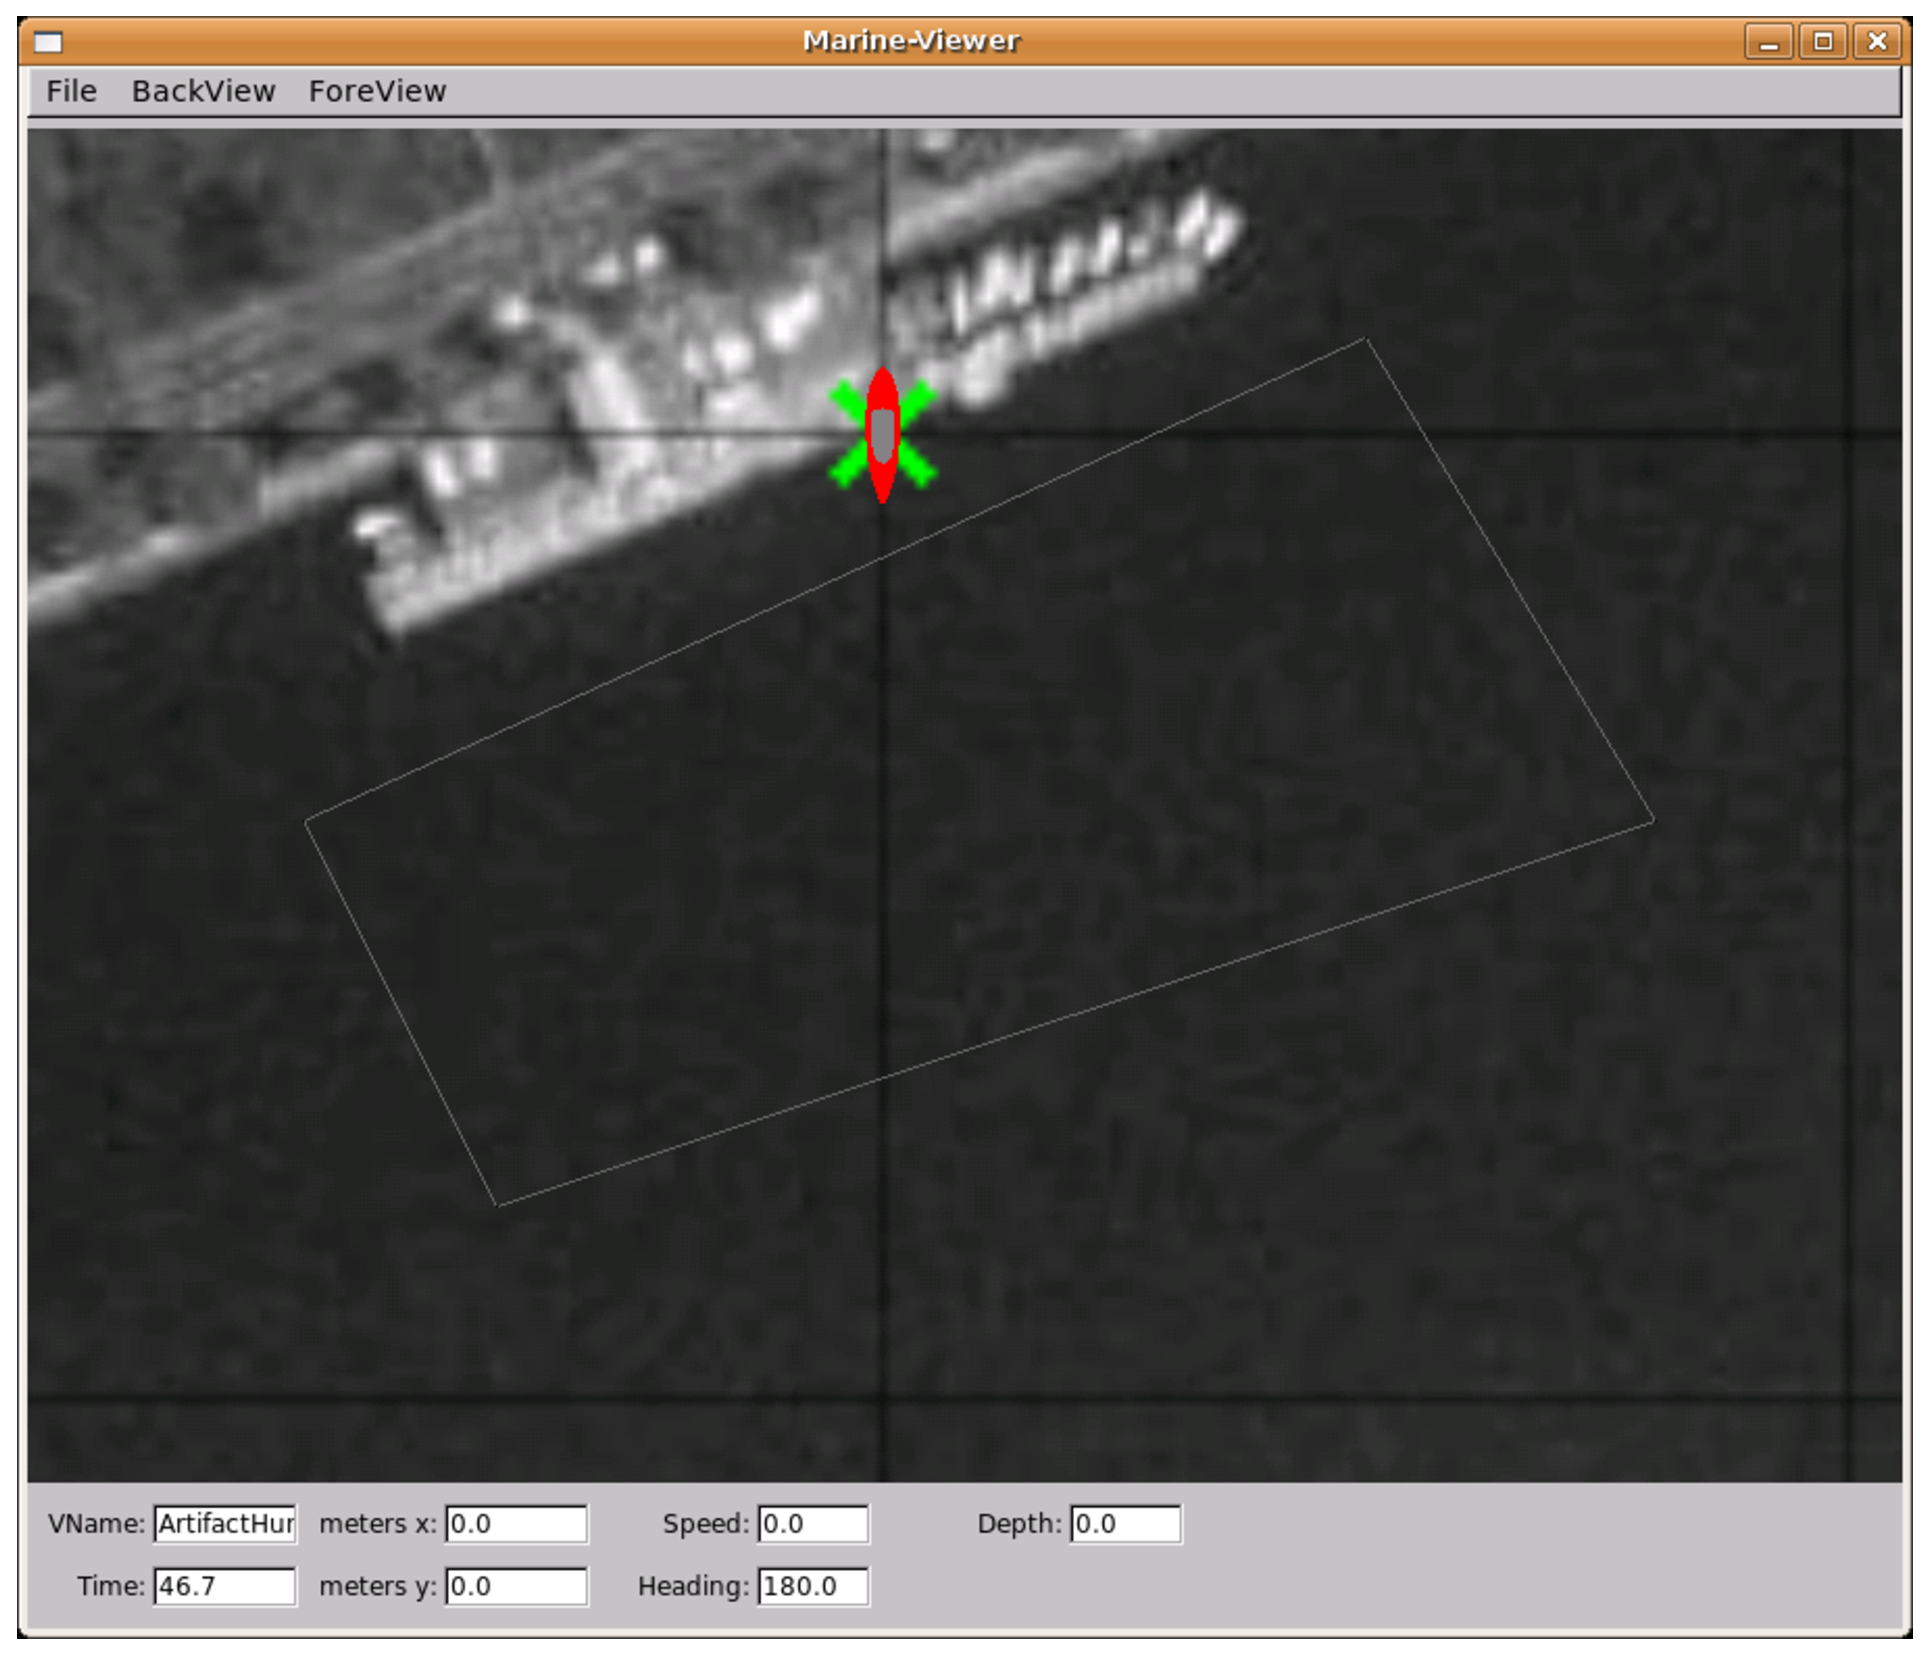
\includegraphics[width=2.5in]{figures/searcharea}
\end{minipage}
\caption{A geographic area (a convex polygon) defined as a search grid.}
\end{figure}

\begin{figure}[ht]
\label{searchgrid}
\begin{minipage}[c]{0.5\textwidth}
  \centering 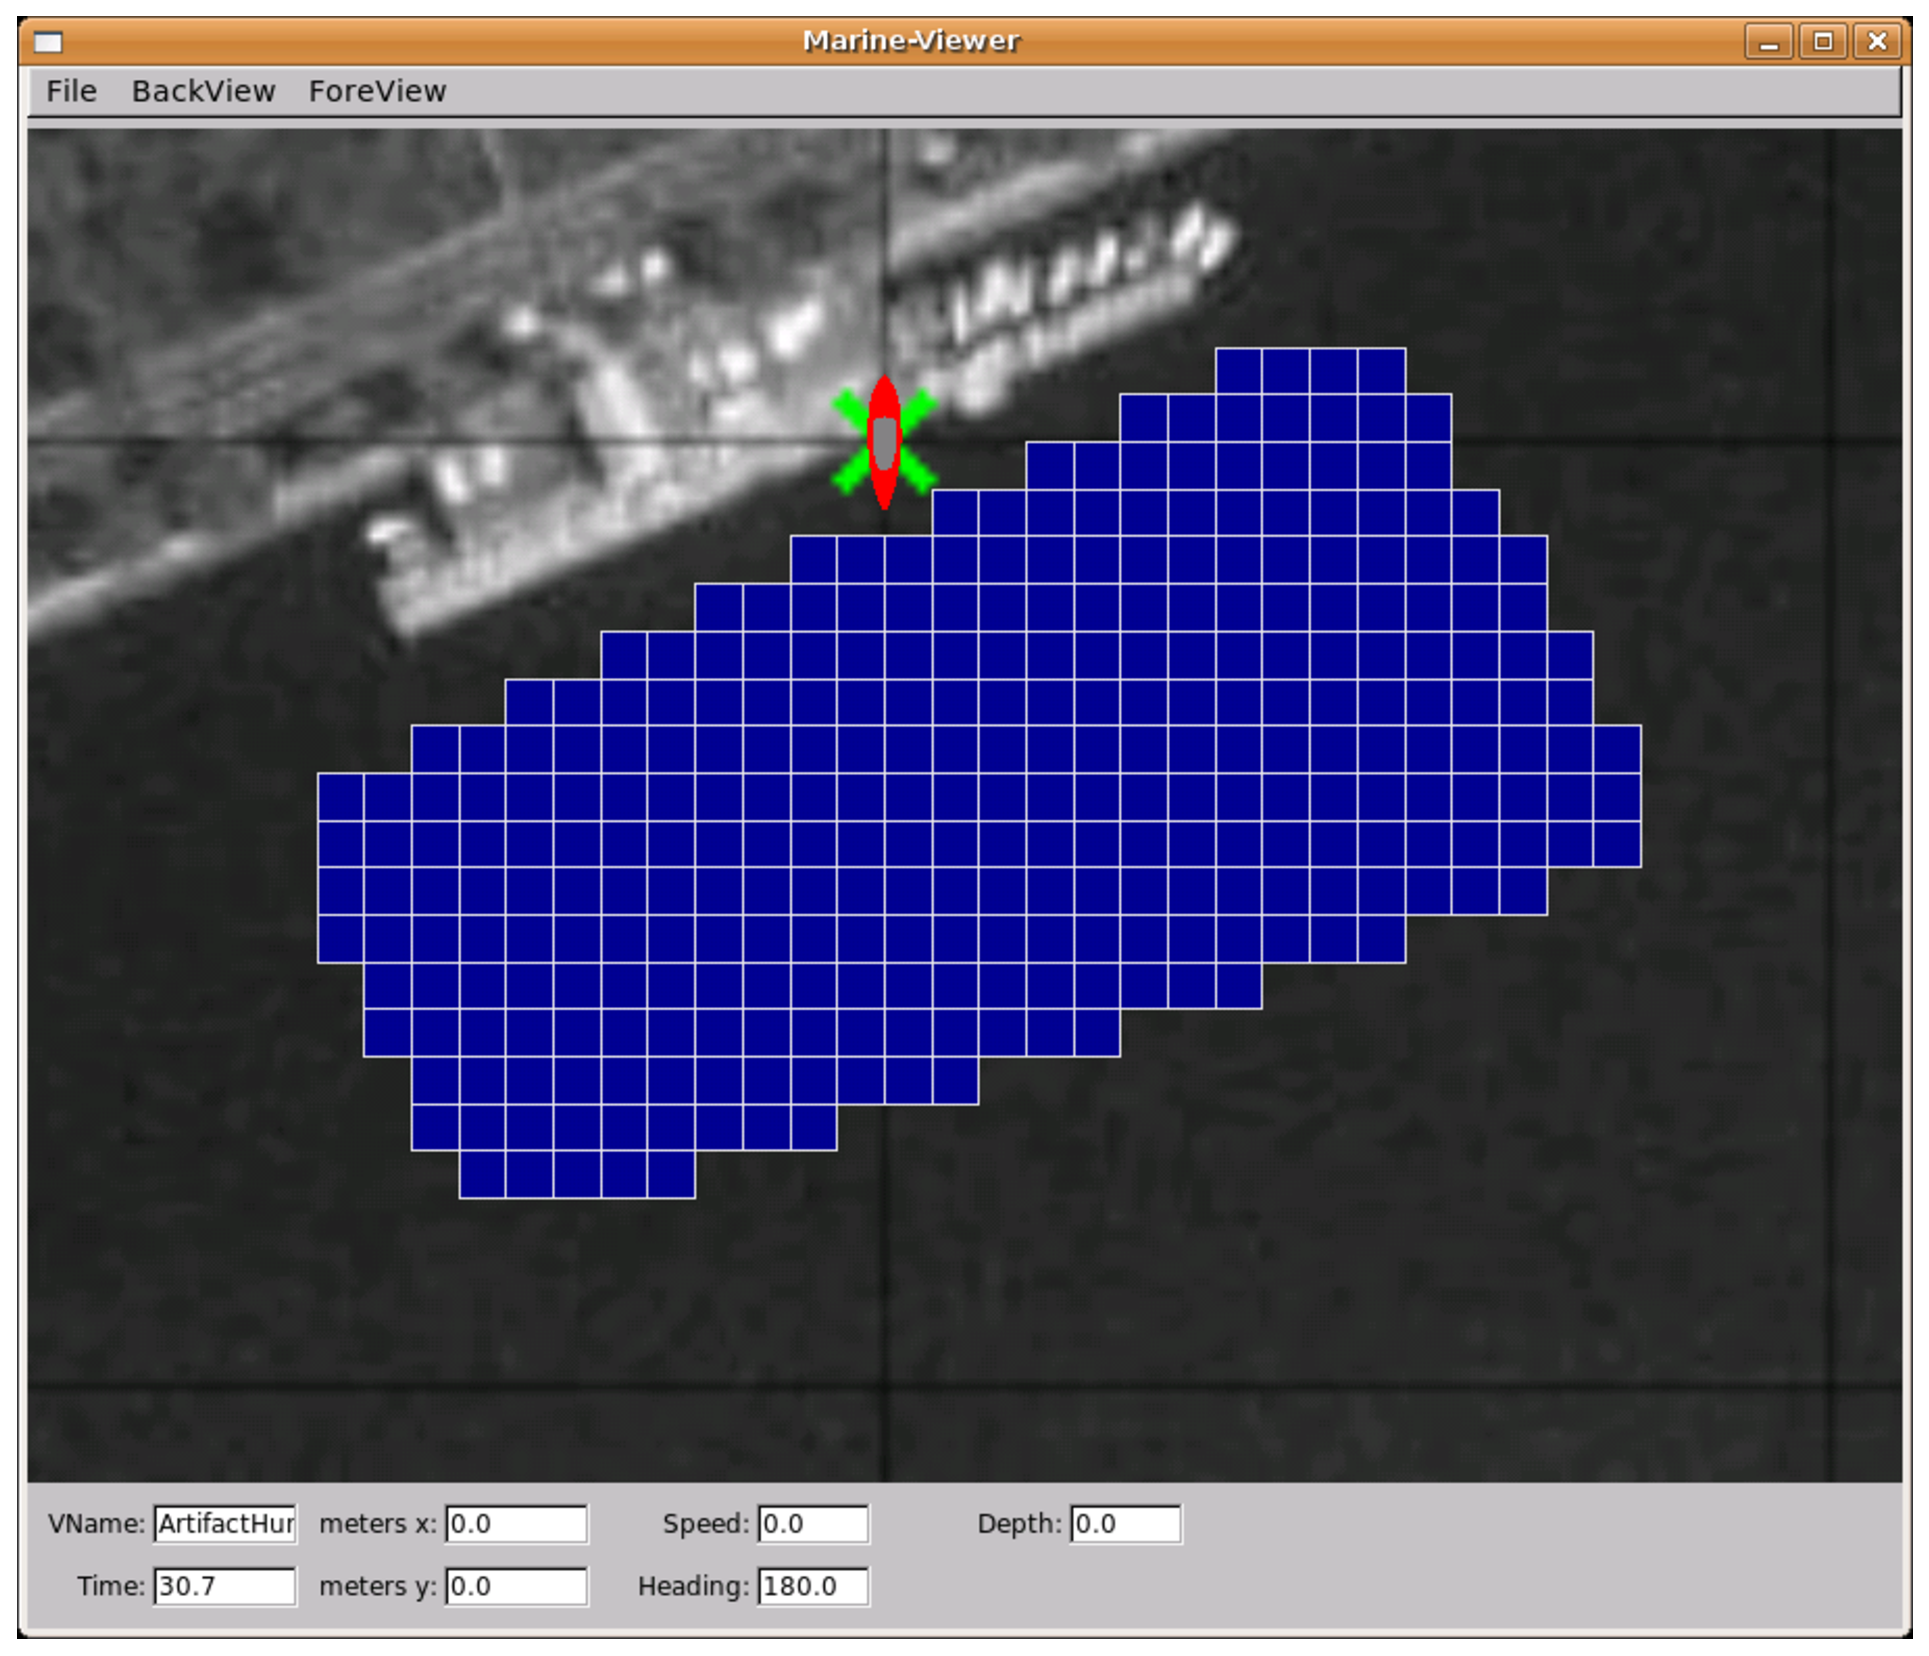
\includegraphics[width=2.5in]{figures/searchgrid}
\end{minipage}%
\caption{A search grid defined over a search area.} 
\end{figure}

There are two main MOOS processes and one IvPHelm behavior that implement the artifact search system.  pSensorSim simulates the output of an imaginary sensor in a simulated artifact field.  pArtifactMapper takes the output of pSensorSim, fuses it with output from other artifact search platforms in the area, and produces a likelihood map of artifacts in the search region.  The IvPHelm behavior, bhv\_SearchGrid, provides desired heading and speed information to the helm to optimize the user's utility function (e.g. mapping an entire field with 95\% confidence in the least amount of time).
% \begin{figure}[ht]
% \begin{minipage}[c]{0.5\textwidth}
%   \centering \includegraphics[width=2.5in]{figures/concept1.eps}
% \end{minipage}%
% \caption{The helm as a process in a MOOS community. \label{conceptone}} 
% \end{figure}


\section{\pmv}
\label{pMarineViewer}
For programming reference, the collaboration diagram for \pmv\ is included in Fig.~\ref{fig:pmvdiagram}.

\img[width=\linewidth]{figures/pmvdiagram}{A collaboration diagram for \pmv}{fig:pmvdiagram}

\subsection{Configuration}
\pmv\ is launched by calling {\tt \pmv\ file.moos} (contrary to the usage instructions, no other arguments are read from the command line).  Also, the file must be named .moos, or it will not be loaded by \pmv.

\subsubsection{MOOS Configuration Block}
The \pmv\ MOOS configuration block looks like:
\scriptsize
\begin{verbatim}
//------------------------------------------
// pMarineViewer config block
{ 
  AppTick   = 4
  CommsTick = 4

  TIF_FILE  = Default.tif  
  VEHICOLOR = nyak200, darkblue
  VEHICOLOR = nyak201, hex, 08, a4, ff
  VEHICOLOR = nyak204, .450, .132, .55
}
\end{verbatim}
\normalsize
\begin{hangpar}{\pin}{\var{TIF\_FILE: }}
Optional.  Default value is ``Default.tif''.  The path to the image file to be used as the background for the display window.  
\end{hangpar}
\begin{hangpar}{\pin}{\var{VEHICOLOR: }}
Optional.  Sets the color of a labelled object.  The format of this string is ``label, \{colorname OR hex[:], ff, ff, ff OR .050, .071, .125\}'' See Appendix~\ref{app:colormap} for a list of color names.
\end{hangpar}

\subsubsection{Background Image Data}
Each tif file should have a .info file with the same name.  Comment lines are prefaced with ``//''.  This text file can have the following entries:
\begin{hangpar}{\pin}{\var{img\_centx and img\_centy: }}
The pixel that represents the origin of the image.  UNITS UNKNOWN.
\end{hangpar}
\begin{hangpar}{\pin}{\var{img\_offset\_x and img\_offset\_y: }}
FEATURE UNDOCUMENTED.
\end{hangpar}
\begin{hangpar}{\pin}{\var{centlat and centlon: }}
The latitude and longitude (in +N and +E degrees) of the center of the image.
\end{hangpar}

For example:
\scriptsize
\begin{verbatim}
img_centx   = 0.495850  
img_centy   = 0.509000
img_meters  = 0.048828
//img_meters  = 0.48828
img_centlat = 42.35849
img_centlon = -71.08759333
\end{verbatim}
\normalsize

\subsection{Menus and Interface}
All \pmv\ keyboard shortcuts are documented in the menu system.  The mouse performs no action in \pmv.

\subsection{MOOS Variables}
\subsubsection{Subscribes}
In all of the requests to plot a figure, if a label is given, requesting to plot that label again with different values will cause the figure to move to that position instead of drawing a duplicate.

\begin{hangpar}{\pin}{\var{AIS\_REPORT and AIS\_REPORT\_LOCAL: }}
An AIS report is a string of the form ``NAME=name, TYPE=type, X=valx, Y=valy, SPD=speed, HDG=heading, DEPTH=depth''.  The name value must match the sending community's name.  All of the variables except type are required for a valid AIS report.  For type, \pmv\ currently knows how to draw types ``kayak'' and ``auv''.  All other types are drawn with a default symbol.
\end{hangpar}
\begin{hangpar}{\pin}{\var{GRID\_CONFIG: }}
Configures \pmv\ to plot a new XYGrid on the display.  The string must be a valid XYGrid configuration string (of the form ``polygon\_string@unit\_string[@initial\_value]'')  A polygon\_string is ``poly[gon]: [label,LABELNAME:] segment\_list''.  A segment\_list is a colon seperated list of comma separated x,y pairs (e.g. 4,5.5:1,2.2).  The unit\_string is the dimensions of the rectangle to place inside the bounding polygon.  It is of the form ``x\_width, y\_width''.  Usually, these are the same value.  The label is used to uniquely identify the grid.
\end{hangpar}
\begin{hangpar}{\pin}{\var{GRID\_DELTA: }}
A string to update the grid.  It is of the form ``LABELNAME@index, old\_val, new\_val[,old\_utility, new\_utility][:index, old\_val, new\_val...]''.
\end{hangpar}
\begin{hangpar}{\pin}{\var{VIEW\_POLYGON: }}
Plots the specified polygon.  The string is a valid XYPolygon initialization string.  Polygons can also be of the form ``radial:xval, yval, radius, num\_points[,snap\_value[,LABELNAME]]'' to approximate a circle.  (An arc can also be plotted, see XYPolygon.cpp for details.)
\end{hangpar}
\begin{hangpar}{\pin}{\var{VIEW\_SEGLIST: }}
Plots the specified seglist.  The string is a valid XYSeglist initialization string.  It is of the form ``[label,LABELNAME:]segment\_list''.  It can also be of the zigzag form (not described here.  See XYSegList.cpp for a description.
\end{hangpar}
\begin{hangpar}{\pin}{\var{VIEW\_POINT and VIEW\_CIRCLE: }}
VIEW\_CIRCLE IS NOT IN SUBSCRIPTION LIST.  VIEW\_POINT plots a dot.  The string is a valid XYCircle initialization string.  It is of the form ``x\_val,y\_val,radius[,LABELNAME]''.
\end{hangpar}
\begin{hangpar}{\pin}{\var{TRAIL\_RESET: }}
Forces \pmv\ to ``forget'' the current trails for any vehicles.
\end{hangpar}
\subsubsection{Publishes}
No MOOSDB writes are created by \pmv.


\section{polyview}
\label{polyview}

\subsection{Configuration}
polyview is launched by calling {\tt polyview image.tif file1 file2\ldots} with arguments in any order.  The image.tif file is the same as the one used by \pmv.  A list of shortcuts for common backgrounds is in Table~\ref{tab:polyviewargs}.  The user and also specify ``-noimg'' to force no background image to load.  All of the other arguments are scanned as text files for Polys, Grids, Arcs, Circles, and Hexagons.

\begin{table}
\renewcommand{\arraystretch}{1.3}
\caption{A list of shortcuts to reference image files in polyview.}
\label{tab:polyviewargs}
\centering
\begin{tabular}{l|l}
\hline
mit OR charles & AerialMIT-1024.tif \\
\hline
wmit OR wireframe OR wf & WireFrameMIT-1024.tif \\
\hline
mb OR monterey & Monterey-2048.tif \\
\hline
mbd & Monterey-2048-30-30-100.tif \\
\hline
\end{tabular}
\end{table}

All readable lines are non-blank and do not begin with `\#'.  Each line is in the format ``key = initialization\_string''.

A Polygon is keyed with ``polygon'', ``points'', or ``radial''.  e.g. ``polygon = polygon:label,A: 0,0: 1,1: 1,0''

A Grid is keyed with ``searchgrid'' (abbreviated ``sgrid'') or ``fullgrid'' (abbreviated ``fgrid'').  It is followed by `=' and then the XYGrid initialization string.  See XYEncoders.cpp, StringToXYGrid for information on the ``fullgrid'' implementation.

An Arc is keyed with ``arc''.  i.e. ``arc = x, y, radius, left\_angle, right\_angle'' (both angles in degrees, 0 is straight up).

A Circle is keyed with ``circle''. i.e. ``circle = x, y, radius[,label]''

A Hexagon is keyed with ``hexagon''. i.e. ``hexagon = x, y, radius\_to\_points''

All of the detected objects are loaded and displayed in the polyview window.

\subsection{Menus and Interface}
The interface for polyview is very similar to the \pmv\ interface.  In the EditMode menu, the various editing operations change the way that a left-click functions in the interface.  The EditMode operations only work on the currently selected object.  The current object is changed in the Polygons menu, or by using + and -.

A new polygon can be created by right-clicking in the interface, or by clicking Polygons-\textgreater Create New.

In the Polygons menu, DumpSpec will output the string that represents the current figure into the terminal window that called polyview.  This is useful for cutting and pasting into text files for other programs (such as moos and behavior files).

NOTES:  Duplicate doesn't seem to work.  The test modes are also undocumented.


\cite{ac90}

\small
\bibliographystyle{plain} 
\bibliography{biblio}


\newpage
\appendices
\section{artfieldgenerator}
\label{app:artfieldgenerator}
artfieldgenerator is a command line tool for generating random artifact fields for testing various behaviors and algorithms.

To use artfieldgenerator:

\scriptsize
{\tt artfieldgenerator poly\_string step\_size num\_artifacts}
\normalsize

\begin{hangpar}{\pin}{\var{poly\_string: }}
A valid polygon initialization string (convex).  All of the artifacts will be contained within this polygon.  Some artifacts, however, may exist outside a search grid, depending on the size of the grid elements.
\end{hangpar}

\begin{hangpar}{\pin}{\var{step\_size: }}
Where to step the X, Y values (e.g. .25 generates values in .25 increments)
\end{hangpar}

\begin{hangpar}{\pin}{\var{num\_artifacts: }}
Number of unique artifacts to generate
\end{hangpar}

The output of artfield generator is written to standard out, so it is often redirected to a file for later use:

\scriptsize
{\tt artfieldgenerator label,A:-60,-40:50,10:80,-40:-40,-80 .25 25 > mines.art}
\normalsize

\section{Tutorial Mission}
\label{app:tutorialmission}
Line break in polygon string is provided for readability only.

File: mission.moos
\scriptsize
\verbatiminput{missions/mission.moos}
\normalsize

\section{Tutorial Behavior}
\label{app:tutorialbehavior}
Line breaks in point list are provided for readability only.

File: artifactsearch.bhv
\scriptsize
\verbatiminput{missions/artifactsearch.bhv}
\normalsize

%\input{sec_bravo_moos}
%\input{sec_charlie_moos}

\end{document}
